\documentclass[twocolumn]{IEEEtran} % LaTeX2e
\usepackage{amssymb,amsmath,graphicx,float}

\begin{document}

\title{Model predictive control of a mobile robot using a successive-linearization approach}

\author{\vskip 1em
Felipe K\"{u}hne, Walter F. Lages and Jo\~{a}o Manoel G. da Silva Jr.\\
\vskip 1em
{\small Federal University of Rio Grande do Sul\\
Department of Electrical Engineering\\
Av. Oswaldo Aranha, 103, Porto Alegre, RS, CEP 90035-190, Brazil\\
{\tt \{kuhne,fetter,jmgomes\}@eletro.ufrgs.br}}}

\maketitle


\begin{abstract}
This paper presents an optimal control scheme for trajectory tracking of a wheeled mobile robot (WMR) with nonholonomic constraints. It is well known that a WMR with nonholonomic constraints cannot be feedback stabilized through continuously differentiable, time-invariant control laws. Using model predictive control (MPC), a discontinuous control law is naturally obtained. One of the main advantages of MPC is the ability to handle constraints (due to state or input limitations) in a straightforward way. Quadratic programming (QP) is used to solve a linear MPC by successive linearization of an error model of the WMR. Simulation results are shown.
\end{abstract}
\begin{keywords}
Wheeled mobile robots, model predictive control, trajectory tracking.
\end{keywords}
\thispagestyle{empty}\pagestyle{empty}


\section{Introduction}\label{sec:intro}
The field of mobile robot control has been the focus of great research effort in the past decades. Besides the apparent simplicity of the kinematic model of a wheeled mobile robot (WMR), the existence of nonholonomic (or non-integrable) constraints turns the design of stabilizing control laws for that systems a great challenge, and due to Brocket's conditions \cite{brockett82}, a continuously differentiable, time-invariant stabilizing feedback control law cannot be obtained. Most works in that direction uses discontinuous (non-smooth) and time-variant control laws (see \cite{bloch89,samson91,canudas92,yamamoto94,murray97} and the references therein). Recent works dealing with robust and adaptive control of WMR's can be found in \cite{oya03,dixon04}.

However, in general, for realistic implementations it is difficult to obtain good performance, due to the constraints on input or state that naturally exist. None of the above cited authors have taken those constraints into account. This can be done in a straightforward way using model predictive control (MPC) schemes. For a WMR this is an important advantage, because the position of the robot can be restricted to belong to a secure region of operation (imagine a WMR crossing a corridor, for example). With input limitations, the control actions can be limited to prevent actuators' saturations.

MPC is a control strategy that uses the model of the system being controlled to obtain an optimal control sequence by minimizing an objective function. At each sample interval, the model provides a prediction of process states over a prediction horizon. Based on that, an objective function is optimized with respect to the future open-loop control system inputs. Although prediction and optimization are computed over a future horizon, only the values of the inputs for the current sample interval are used and the same procedure is repeated at the next sample instant. This mechanism is known as {\it moving} or {\it receding horizon} strategy, in reference to the way in which the time window considered in the calculations shifts forward from one time step to the next.

For complex constrained multivariable control problems, MPC has become the accepted standard in the process industries \cite{bemporad02}. It was very well used in such cases, specially where plants being controlled are sufficiently {\em slow} to permit its implementation \cite{mayne98}. However, for systems with fast and/or nonlinear dynamics, like the WMR's, the implementation of such technique remains fundamentally limited in applicability, due to large amount of {\em on-line} computation required \cite{cannon00}. In this paper we overcome this problem by using a successive-linearization approach, where a linear MPC is solved by quadratic programming (QP) problem. With some simulations results, it is shown that even a real-time implementation is possible. Although MPC is not a new control method, works dealing with MPC of WMR's are recent and sparse \cite{ollero91,rico99,essen01}.

The remainder of this paper is organized as follows: in the next section the kinematic model of the WMR is shown. The MPC algorithm is depicted in Section \ref{sec:mpc}. Simulation results in {\sc matlab} are shown in Section \ref{sec:simulations}, where an eight-like trajectory is used as reference. The paper finishes with the conclusions. 


\section{Kinematic model of the WMR}\label{sec:model}
In this section the kinematic model of the WMR is described. A mobile robot made up of a rigid body and non deformable wheels is considered and depicted in Fig. \ref{fig:robot}. It is assumed that the vehicle moves without slipping in an horizontal ground. The kinematics of the WMR is given by:
\begin{equation}\label{eqn:model}
	\left\{
		\begin{aligned}
			\dot x	  &= v\cos\theta \\
			\dot y	  &= v\sin\theta \\
			\dot \theta &= w \\
		\end{aligned}
	\right.
\end{equation}

The state vector
\begin{equation*}
	{\bf x}\triangleq[x~~y~~\theta]^T
\end{equation*}
describes the configuration (position and orientation) of the center of mass $C$ of the robot with respect to a global inertial frame $\{O,X,Y\}$, and
\begin{equation*}
	{\bf u}\triangleq[v~~w]^T
\end{equation*}
is the manipulated (control) variables, where $v$ and $w$ are the forward and angular velocities, respectively.
\begin{figure}[t]\begin{center}
    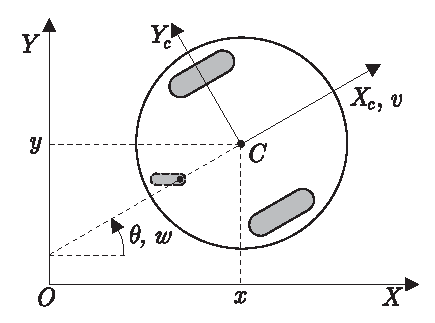
\includegraphics[width=.67\linewidth]{Figures/robot.eps}
    \caption{Kinematic model of the WMR.}
    \label{fig:robot}
\end{center}\end{figure}

An error model between (\ref{eqn:model}) and a reference model,
\begin{equation}\label{eqn:refmodel}
	\left\{
		\begin{aligned}
			\dot x_r	  &= v_r\cos\theta_r \\
			\dot y_r	  &= v_r\sin\theta_r \\
			\dot \theta_r &= w_r \\
		\end{aligned}
	\right.,
\end{equation}
can be described as follows:
\begin{equation}\label{eqn:errormodel}
	\left\{
		\begin{aligned}
			\dot e_x	    &= e_v\cos\theta_r \\
			\dot e_y	    &= e_v\sin\theta_r \\
			\dot e_\theta &= e_w \\
		\end{aligned}
	\right.
\end{equation}
with:
\begin{equation*}
	{\bf e}_{\bf x} \triangleq \begin{bmatrix}
		e_x \\ e_y \\ e_\theta
	\end{bmatrix} =
	\begin{bmatrix}
		\cos\theta_r  & \sin\theta_r & 0 \\
		-\sin\theta_r & \cos\theta_r & 0 \\
		0		    & 0		    & 1
	\end{bmatrix} 
	\begin{bmatrix}
		x-x_r \\ y-y_r \\ \theta-\theta_r
	\end{bmatrix}
\end{equation*}
and
\begin{equation*}
	{\bf e}_{\bf u} \triangleq {\bf u} - {\bf u}_r = \begin{bmatrix}
		e_v \\ e_w
	\end{bmatrix} =
	\begin{bmatrix}
		v-v_r \\ w-w_r
	\end{bmatrix}
\end{equation*}

Indeed, the convergence of ${\bf x}$ to ${\bf x}_r$ is equivalent to the convergence of ${\bf e_x}$ to the set ${\cal O}=\{{\bf x}|(e_x,e_y,e_\theta)=(0,0,2\pi n)\},n\in \{0,\pm1,\pm2,\ldots\}$.

Discretizing (\ref{eqn:errormodel}) by the Euler method, i.e.,
\begin{equation*}
	\dot{\bf e}_{\bf x} \approx \frac{{\bf e_x}(k+1)-{\bf e_x}(k)}{T},
\end{equation*}
where $T$ is the sampling period, we have the following nonlinear, discrete-time error model:
\begin{equation}\label{eqn:discreteerror}
	\left\{
		\begin{aligned}
			e_x(k+1)	    &= e_x(k) + e_v(k)\cos\theta_r(k)T \\
			e_y(k+1)	    &= e_y(k) + e_v(k)\sin\theta_r(k)T \\
			e_\theta(k+1) &= e_\theta(k) + e_w(k)T \\
		\end{aligned}
	\right.,
\end{equation}
where $k$ is the sampling time. It must be noted that actually there are only reference states. The reference controls ${\bf u}_r$ can be obtained, using ${\bf x}_r$, with:
\begin{align*}
	v_r(k) &= \frac{x_r(k+1)-x_r(k)}{\cos\theta_r(k) T}, \\
	w_r(k) &= \frac{\theta_r(k+1)-\theta_r(k)}{T}
\end{align*}

Now, it is possible to reformulate the error model as a linear, time-variant model. Considering (\ref{eqn:discreteerror}) equal to \mbox{${\bf x}(k+1)=f({\bf x}(k),{\bf u}(k))$}, we have:
\begin{equation}\label{eqn:error2}
	{\bf e}_{\bf x}(k+1) = {\bf A}(k){\bf e_x}(k) + {\bf B}(k){\bf e_u}(k),
\end{equation}
where the matrices ${\bf A}(k)$ and ${\bf B}(k)$ are the jacobians of $f({\bf x}(k),{\bf u}(k))$ with relation to ${\bf e_x}(k)$ and ${\bf e_u}(k)$, respectively, evaluated at the reference point $({\bf x}_r(k),{\bf u}_r(k))$,
\begin{align*}
	{\bf A}(k) &\triangleq \left.\frac{\partial f}{\partial{\bf e}_{\bf x}}\right|_{\begin{smallmatrix}{\bf x}(k)={\bf x}_r(k) \\ {\bf u}(k)={\bf u}_r(k) \end{smallmatrix}} = \begin{bmatrix}
		1 & 0 & -v_r(k)\sin\theta_r(k)T \\
		0 & 1 &  v_r(k)\cos\theta_r(k)T \\
		0 & 0 & 1
	\end{bmatrix}, \\
	{\bf B}(k) &\triangleq \left.\frac{\partial f}{\partial{\bf e}_{\bf u}}\right|_{\begin{smallmatrix}{\bf x}(k)={\bf x}_r(k) \\ {\bf u}(k)={\bf u}_r(k) \end{smallmatrix}} = \begin{bmatrix}
		\cos\theta_r(k)T & 0 \\
		\sin\theta_r(k)T & 0 \\
		0 			  & T
	\end{bmatrix}
\end{align*}

Equation (\ref{eqn:error2}) is a discrete-time, time-variant, linear error model for the WMR, and will be used in the MPC algorithm for the QP problem resolution.

Bloch and McClamroch \cite{bloch89} have shown that the nonlinear, nonholonomic system of (\ref{eqn:model}) is fully controllable, i.e., it can be steered from any initial state to any final state in finite time by using finite inputs. It is easy to note that the linearization about a stationary operating point, when the car is motionless, is not controllable. However, this linearization becomes controllable as long as the control inputs ${\bf u}$ are existing \cite{samson91}. This implies that the tracking of a reference trajectory would be possible with linear MPC \cite{essen01}.


\section{The MPC Algorithm}\label{sec:mpc}
As cited in Section \ref{sec:intro}, the essence of a MPC scheme is to optimize, over the control inputs, predictions of process behavior. Such prediction is accomplished using a process model over a finite time interval, called the {\em prediction horizon}. At each sample time, the model predictive controller generates an optimal control sequence by solving a minimization problem. The first element of this sequence is applied to the plant being controlled. The problem is solved again at the next time interval using updated process measurements and a shifted horizon.

In this work, for simplicity we assume that the states of the plant are always available for measure, and that there are no plant/model mismatch (the linearized plant and the linearized model are exactly the same). Also, in order to design the linear controller, it is assumed that the pair $({\bf A}(k),{\bf B}(k))$ is always (at any $k$) stabilizable.

Usually, the optimization problem can be written as:
\begin{equation*}
	\min_{\bf\varphi}\left\{\Phi_k\right\}
\end{equation*}
subject to:
\begin{equation*}\label{eqn:constr}
	{\bf\varphi}_{min} \leq {\bf\varphi} \leq {\bf\varphi}_{max}
\end{equation*}

$\Phi_k$ is the so called {\em cost function} and usually, for linear systems, takes a quadratic form. ${\bf\varphi}$ is the free variable in the optimization, and ${\bf\varphi}_{min}$ and ${\bf\varphi}_{max}$ are its inferior and superior limits, respectively.

The cost function to be minimized is the following:
\begin{multline}\label{eqn:cost}
	\Phi_k = \sum_{j=1}^{N}{\bf e}_{\bf x}^T(k+j|k){\bf Q}{\bf e}_{\bf x}(k+j|k) + \\ + {\bf e}_{\bf u}^T(k+j-1|k){\bf R}{\bf e}_{\bf u}(k+j-1|k),
\end{multline}
where $N$ is the prediction horizon and ${\bf Q}$, ${\bf R}$ are positive definite weighting matrices. The free variable is, in this case, the control error ${\bf e_u}$. The notation $a(k+j|k)$ indicates the value of $a$ at the instant $k+j$ predicted at instant $k$.

\subsection{Derivation of the QP problem}\label{sec:qp}
In the following, the MPC optimization problem will be recast as a standard QP problem. Equation (\ref{eqn:cost}) can be rewritten as:
\begin{equation}\label{eqn:cost2}
	\Phi_k = \overline{\bf e}_{\bf x}^T\overline{\bf Q}\overline{\bf e}_{\bf x} + \overline{\bf e}_{\bf u}^T\overline{\bf R}\overline{\bf e}_{\bf u},
\end{equation}
with
\begin{align*}
	\overline {\bf e}_{\bf x} &\triangleq \begin{bmatrix}
		{\bf e}_{\bf x}(k+1|k) \\ {\bf e}_{\bf x}(k+2|k) \\ \vdots \\ {\bf e}_{\bf x}(k+N|k) 
	\end{bmatrix} \quad
	\overline{\bf e}_{\bf u} \triangleq \begin{bmatrix}
		{\bf e_u}(k|k)  \\ {\bf e_u}(k+1|k) \\ \vdots \\ {\bf e_u}(k+N-1)
	\end{bmatrix} \\
	\overline {\bf Q} &\triangleq \begin{bmatrix}
		{\bf Q} & {\bf 0} & \cdots & {\bf 0} \\
		{\bf 0} & {\bf Q} & \cdots & {\bf 0} \\
		\vdots  & \vdots  & \ddots & \vdots  \\
		{\bf 0} & {\bf 0} & \cdots & {\bf Q} \\
	\end{bmatrix} \qquad
	\overline {\bf R} \triangleq \begin{bmatrix}
		{\bf R} & {\bf 0} & \cdots & {\bf 0} \\
		{\bf 0} & {\bf R} & \cdots & {\bf 0} \\
		\vdots  & \vdots  & \ddots & \vdots  \\
		{\bf 0} & {\bf 0} & \cdots & {\bf R} \\
	\end{bmatrix}
\end{align*}

By means of the {\em Superposition Principle} for the time-variant linear model (\ref{eqn:error2}), the following expression can be derived:
\begin{multline*}
	{\bf e}_{\bf x}(k+j|k) = {\bf A}^j(k){\bf e}_{\bf x}(k|k) + \\ + \sum_{i=0}^{j-1}{\bf A}^{j-1-i}(k+i){\bf B}(k+i){\bf e}_{\bf u}(k+i|k)
\end{multline*}
and the state error $\overline{\bf e}_{\bf x}$ takes the form:
\begin{equation}\label{eqn:exbar}
	\overline{\bf e}_{\bf x}=\overline{\bf A}{\bf e}_{\bf x}(k|k)+{\bf S}\overline{\bf e}_{\bf u},
\end{equation}
where $\overline{\bf A} \triangleq [{\bf A}(k)~~{\bf A}^2(k)~~\cdots~~{\bf A}^N(k)]^T$ and
{\small
	\begin{equation*}
		{\bf S} \triangleq \begin{bmatrix}
			{\bf B}(k)                 & {\bf 0} 					& \cdots & {\bf 0}       \\
			{\bf A}(k){\bf B}(k)       & {\bf B}(k+1)      			& \cdots & {\bf 0}       \\
			\vdots	                 & \vdots		     		& \ddots & \vdots        \\
			{\bf A}^{N-1}(k){\bf B}(k) & {\bf A}^{N-2}(k+1){\bf B}(k+1) & \cdots & {\bf B}(k+N-1)
		\end{bmatrix}
	\end{equation*}
}

With (\ref{eqn:cost2}) and (\ref{eqn:exbar}) at hands, and after some algebraic manipulations, we can rewrite the cost function (\ref{eqn:cost}) in a standard quadratic form:
\begin{equation}
	\Phi_k = \frac{1}{2}\overline{\bf e}_{\bf u}^T{\bf H}\overline{\bf e}_{\bf u} + {\bf f}^T\overline{\bf e}_{\bf u}
\end{equation}
with
\begin{align*}
	{\bf H} &\triangleq 2\left({\bf S}^T\overline{\bf Q}{\bf S}+\overline{\bf R}\right) \\
	{\bf f} &\triangleq 2{\bf S}^T\overline{\bf Q}\overline{\bf A}{\bf e}_{\bf x}(k|k)
\end{align*}

The matrix ${\bf H}$ is the {\em Hessian} matrix, and must be positive definite. It describes the quadratic part of the cost function, and the vector ${\bf f}$ describes the linear part. 

Now it is possible to define constraints, for example, in the control action ${\bf u}(k)$, or in vector form, $\overline {\bf u}$. So, we have the following constraint:
\begin{equation}\label{eqn:uconstr}
	\overline{\bf u}_{min} \leq \overline{\bf u} \leq \overline{\bf u}_{max},
\end{equation}
with the limits 
% ${\bf u}_{min}(k)=[v_{min}(k)~w_{min}(k)]^T$, ${\bf u}_{max}(k)=[v_{max}(k)~w_{max}(k)]^T$ and
\begin{equation*}
	{\bf u}_{min}(k) = \begin{bmatrix}
		v_{min}(k) \\ w_{min}(k)
	\end{bmatrix} \quad 
	{\bf u}_{max}(k) = \begin{bmatrix}
		v_{max}(k) \\ w_{max}(k)
	\end{bmatrix}
\end{equation*}
and
\begin{align*}
	\overline{\bf u}_{min} &\triangleq \begin{bmatrix}
		{\bf u}_{min}(k) \\ {\bf u}_{min}(k+1) \\ \vdots \\ {\bf u}_{min}(k+N-1)
	\end{bmatrix} \\
	\overline{\bf u}_{max} &\triangleq \begin{bmatrix}
		{\bf u}_{max}(k) \\ {\bf u}_{max}(k+1) \\ \vdots \\ {\bf u}_{max}(k+N-1)
	\end{bmatrix}
\end{align*}

In this case, the free variable in the optimization is the vector $\overline{\bf e}_{\bf u}$, and the constraint (\ref{eqn:uconstr}) must be rewritten with respect to this variable (remembering that ${\bf e_u}(k)={\bf u}(k)-{\bf u}_r(k)$):
\begin{equation*}
	\overline{\bf u}_{min} - \overline{\bf u}_r \leq \overline{\bf e}_{\bf u} \leq \overline{\bf u}_{max} - \overline{\bf u}_r
\end{equation*}
where
\begin{equation*}
	\overline{\bf u}_r \triangleq \begin{bmatrix}
		{\bf u}_r(k) \\ {\bf u}_r(k+1) \\ \vdots \\ {\bf u}_r(k+N-1)
	\end{bmatrix}
\end{equation*}


\section{Simulation results}\label{sec:simulations}
In this section, simulation results are shown for the MPC applied to a WMR. The optimization problem has been solved with the {\sc matlab} routine {\tt quadprog}. The data used for the simulation are: ${\bf x}(0)=[-0.8~~1~~\pi]^T$ (initial configuration of the WMR), ${\bf Q}={\bf I}_{3\times 3}$, ${\bf R}={\bf I}_{2\times 2}$ and $N=3$. Also, control contstraints were imposed: $v_{min}=0.2 m/s$, $v_{max}=0.4 m/s$, $w_{min}=-0.4 rad/s$ and $w_{max}=0.4 rad/s$. It can be seen that the state converges to the references. In Fig. \ref{fig:traj8} and \ref{fig:states}, the dash-dotted line stands for the reference trajectory of the states. Fig. \ref{fig:errors} shows the errors of the states converging to zero. The most interesting one is Fig. \ref{fig:controls}. It can be clearly seen that the control inputs obey the limits imposed by the constraints. As the state errors converge to zero (Fig. \ref{fig:errors}), one could say that the value of the cost function must converges to zero too. This fact can be observed in Fig. \ref{fig:cost}.
\begin{figure}\begin{center}
    \includegraphics[width=\linewidth]{Figures/traj8.eps}
    \caption{Trajectory covered by the WMR, in the $XY$ plane.}
    \label{fig:traj8}
\end{center}\end{figure}
\begin{figure}\begin{center}
    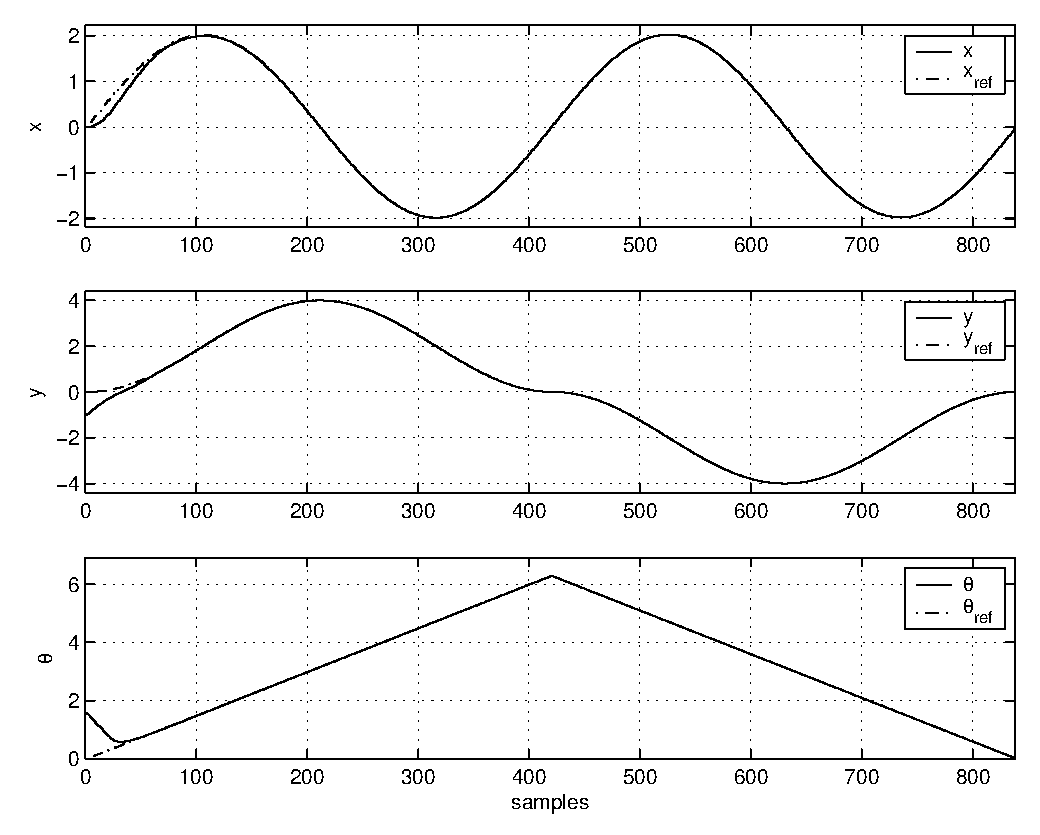
\includegraphics[width=\linewidth]{Figures/states.eps}
    \caption{States $x$, $y$ and $\theta$ of the WMR.}
    \label{fig:states}
\end{center}\end{figure}
\begin{figure}\begin{center}
    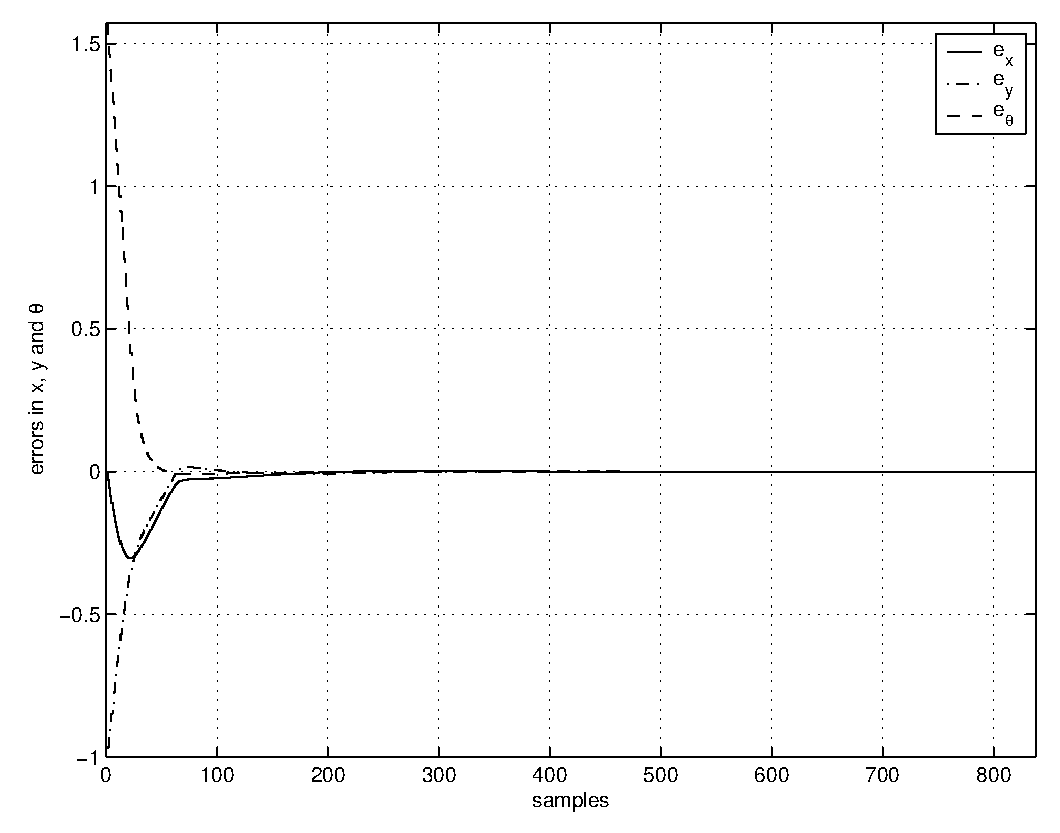
\includegraphics[width=\linewidth]{Figures/errors.eps}
    \caption{Errors between states and references.}
    \label{fig:errors}
\end{center}\end{figure}
\begin{figure}\begin{center}
    \includegraphics[width=\linewidth]{Figures/controls.eps}
    \caption{Controls bounded by the constraints (dotted lines for unconstrained case).}
    \label{fig:controls}
\end{center}\end{figure}
\begin{figure}\begin{center}
    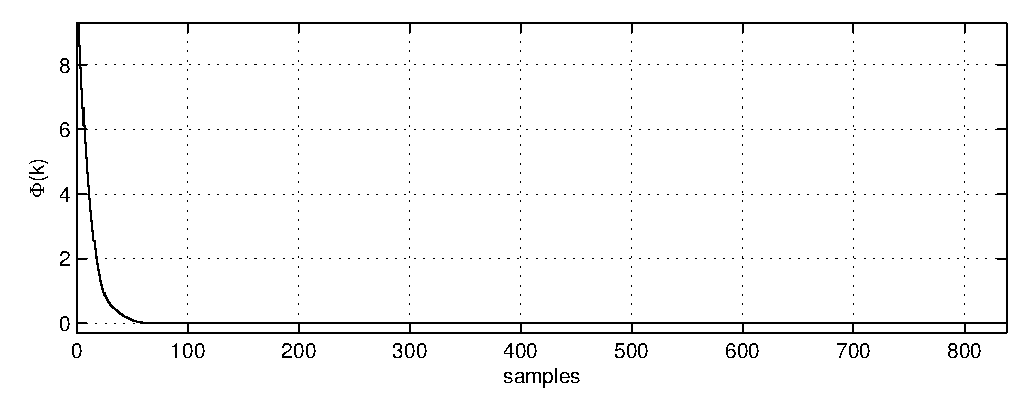
\includegraphics[width=\linewidth]{Figures/cost.eps}
    \caption{Value of the cost function $\Phi_k$.}
    \label{fig:cost}
\end{center}\end{figure}

\section{Conclusion}\label{sec:conclusions}
This paper has presented the application of MPC to a nonholonomic WMR, represented by means of a kinematic model. It was shown the solution of the optimization problem through a standard QP method. Constraints were imposed on the control variables, which obeyed it perfectly. Such research will obviously continue, and the authors' main objective is real-time simulations of nonlinear model predictive control (NMPC) applied to WMR's.


\subsection*{Acknowledgments}
The authors gratefully acknowledge the financial support from CAPES.


\begin{thebibliography}{}

% This is a book
\bibitem{brockett82}
R. W. Brockett, 
{\em New Directions in Applied Mathematics},
Springer-Verlag, New York, 1982.

\bibitem{bloch89}
A. M. Bloch and N. H. McClamroch,
"Control of mechanical systems with classical nonholonomic constraints",
{\em Proceedings of American Conference on Decision and Control\/}, Tampa, Florida, pp. 201--205, 1989.

\bibitem{samson91}
C. Samson and K. Ait-Abderrahim,
"Feedback control of a nonholonomic wheeled cart in cartesian space",
{\em Proceedings of IEEE Int. Conf. on Robotics and Automation\/}, Sacramento, California, pp. 1136--1141, 1991.

% This is an magazine article
\bibitem{canudas92}
C. Canudas de Wit and O. J. S\o rdalen, 
"Exponential stabilization of mobile robots with nonholonomic constraints",
{\em IEEE Trans. Automatic Control\/}, vol. 37(11), pp. 1791--1797, 1992.

\bibitem{yamamoto94}
Y. Yamamoto and X. Yun, 
"Coordinating locomotion and manipulation of a mobile manipulator",
{\em IEEE Trans. Automatic Control\/}, vol. 39(6), pp. 1326--1332, 1994.

\bibitem{murray97}
R. T. McCloskey and R. M. Murray, 
"Exponential stabilization of driftless control systems using homogeneous feedback",
{\em IEEE Trans. Automatic Control\/}, vol. 42(5), pp. 614--628, 1997.

\bibitem{oya03}
M. Oya, C. Y. Su and R. Katoh, 
"Robust adaptive motion/force tracking control of uncertain nonholonomic mechanical systems",
{\em IEEE Trans. Robotics and Automation\/}, vol. 19(1), pp. 175--181, 2003.

\bibitem{dixon04}
W. E. Dixon, M. S. de Queiroz, D. M. Dawson and T. J. Flynn, 
"Adaptive tracking and regulation of a wheeled mobile robot with controller/update law modularity",
{\em IEEE Trans. Control Systems Technology\/}, vol. 12(1), pp. 138--147, 2004.

\bibitem{bemporad02}
A. Bemporad, F. Borrelli and M. Morari, 
"Model predictive control based on linear programming -- The explicit solution",
{\em IEEE Trans. Automatic Control\/}, vol. 47(12), pp. 1974--1985, 2002.

\bibitem{mayne98}
D. Q. Mayne, J. B. Rawlings, C. V. Rao and P. O. M. Scokaert, 
"Constrained model predictive control: Stability and optimality",
{\em Automatica\/}, vol. 36(12), pp. 789--814, 1998.

\bibitem{cannon00}
M. Cannon and B. Kouvaritakis, 
{\em Continuous-time predictive control of constrained nonlinear systems},
pp. 204--215, Nonlinear model predictive control, Progress in systems and control theory, Vol. 26,
F. Allg\"{o}wer, A. Zeng, editors, Birkh\"{a}user Verlag, Basel/Switzerland, 2000.

\bibitem{allgower99}
F. Allgower, T. A. Badgwell, J. S. Qin, J. B. Rawlings and S. J. Wright, 
{\em Nonlinear Predictive Control and Moving Horizon Estimation -- An Introductory Overview},
Chapter 12, pp. 391--449, Advances In Control: Highlights of ECC'99,
P. M. Frank, editor, Springer-Verlag, New York, 1999.

\bibitem{garcia89}
C. E. Garc\'{i}a, D. M. Prett and M. Morari, 
"Model predictive control: Theory and practice -- A survey",
{\em Automatica\/}, vol. 25(3), pp. 335--348, 1989.

\bibitem{ollero91}
A. Ollero and O. Amidi,
"Predictive path tracking of mobile robots. Application to the CMU Navlab",
{\em Proceedings of 5th. IEEE Int. Conf. on Advanced Robotics\/}, Pisa, Italy, pp. 1081--1086, 1991.

\bibitem{rico99}
J. E. Normey-Rico, J. G\'{o}mez-Ortega and E. F. Camacho, 
"A Smith-predictor-based generalised predictive controller for mobile robot path-tracking",
{\em Control Engineering Practice\/}, vol. 7, pp. 729--740, 1999.

% This is a congress proceeding
\bibitem{essen01}
H. V. Essen and H. Nijmeijer,
"Non-linear model predictive control of constrained mobile robots",
{\em Proceedings of European Control Conference\/}, Porto, Portugal, pp. 1--12, 2001.

\end{thebibliography}


\end{document}


